\section{Performance Evaluation}

Two platforms were for performance evaluation of our novel \textit{PackDrop} scheduler:
i) A tightly coupled \textit{Supercomputer} with $24$ (in $2$ separate NUMA nodes) PEs per node, using an Infiniband interconnection supported by Intel's Parallel Studio XE implementation of \texttt{MPI} (v2017.4).
ii) A smaller \textit{Cluster} with $4$ PEs per node, using a Gigabit Ethernet interconnection.
Details of both platforms are available on Table~\ref{tab:ptinfo}.

\begin{table}[ht]
    \centering
	\begin{tabular}{c|c|c}
	Node Info.	 		& Supercomputer 		& Cluster \\ \hline
        CPUs	   			& $2\times12$ 			& $4$ \\
        Intel Xeon			& E5-2695v2 			& X3440\\
        CPU Freq.  			& $2.4$GHz   			& $2.53$GHz\\
        RAM        			& $64$GB			& $16$GB\\
        Network 			& Infiniband FDR 		& Gigabit Ethernet\\
        OS      			& RedHat Linux 6.4 		& Ubuntu 14.04\\
        \texttt{GCC}			& $5.3.1$			& $5.4.0$\\
        \texttt{Charm++} 		& $6.8.1$ 			& $6.8.1$\\
        \texttt{MPI}			& $3.1.0$			& -\\
        \texttt{GCC} Flags		& \texttt{-std=c++11 -O3} 	& \texttt{-std=c++11 -O3} \\
	\end{tabular}
    \caption{Platform Information of each Node from Supercomputer and Cluster evaluations.}
    \label{tab:ptinfo}
\end{table}

Ahead we'll present the metrics used to compare our new global rescheduling strategy with \textit{Greedy}, \textit{Refine} and \textit{Distributed}.
Then, we'll discuss results obtained in both platforms descripted in Table~\ref{tab:ptinfo} and the scalability of our proposed solution.
All raw data of our results, as well as parsing scripts for analysis are publicly available\footnote{Available at: \texttt{https://github.com/OMMITED-FOR-BLIND-REVIEW}.}.

\subsubsection*{Metrics}

\textit{Application time} is one of the most relevant metrics to evaluate load balancers in \texttt{Charm++}.
Since migrations may induce high overhead and impact communication costs, a bad algorithm may finish fast, but increase imbalance, and thus, application time.

\textit{Load balancer decision time}, although not the most relevant for the application itself, the decision time is an indicator of its scalability.
Some centralized schedulers, such as \textit{Greedy}, work very well on local machines, with a reasonable data input.
However, when executing on distributed memory environments, the scalability of centralized strategies is limited.

\subsection{Evaluation on Cluster}

All experiments executed on cluster were compiled with \texttt{Charm++} using the \texttt{--with-production} option, combined with the specifications detailed on Table~\ref{tab:ptinfo}.
$32$ homogeneous compute nodes were used, with a total of $128$ PEs.
In addition to previously mentioned schedulers, \textit{Dummy} was added as the representative of a situation with no remap of tasks, it only aggregates the information a centralized strategy needs (its cost is the base for every centralized strategy).

\subsubsection*{Evaluation with Synthetic Load}

\textit{LB Test} experiments had a total of $18990$ \textit{tasks}, executed over $150$ iterations, performing load balance every $40$ iterations.
\textit{Task} loads vary from $30$ms to $9000$ms, which provides reasonable imbalance of load, causing global rescheduling to be useful in this case.
Ring, 2D mesh and 3D mesh communication topologies were used to provide different levels of migration impact and communication cost.

\begin{table}[t]
	\centering
	\begin{tabular}{l | c  c  c}
    	Scheduler & Time (Ring) & Time (2D) & Time (3D) \\ \hline
        Distributed & $47.49298$s & $48.64839$s & $49.05481$s \\
        Greedy & $46.54101$s & $49.56052$s & $51.06850$s \\
        Dummy & $52.43016$s & $53.17254$s & $53.94068$s \\
        PackDrop & $46.81598$s & $47.37120$s & $47.97426$s \\
        Refine & $45.49095$s & $46.29277$s & $47.21924$s \\		
	\end{tabular}
    \caption{LB Test mean application time on the cluster execution.}
    \label{tab:lbtest:apptime}
\end{table}

\begin{figure}
	\centering
    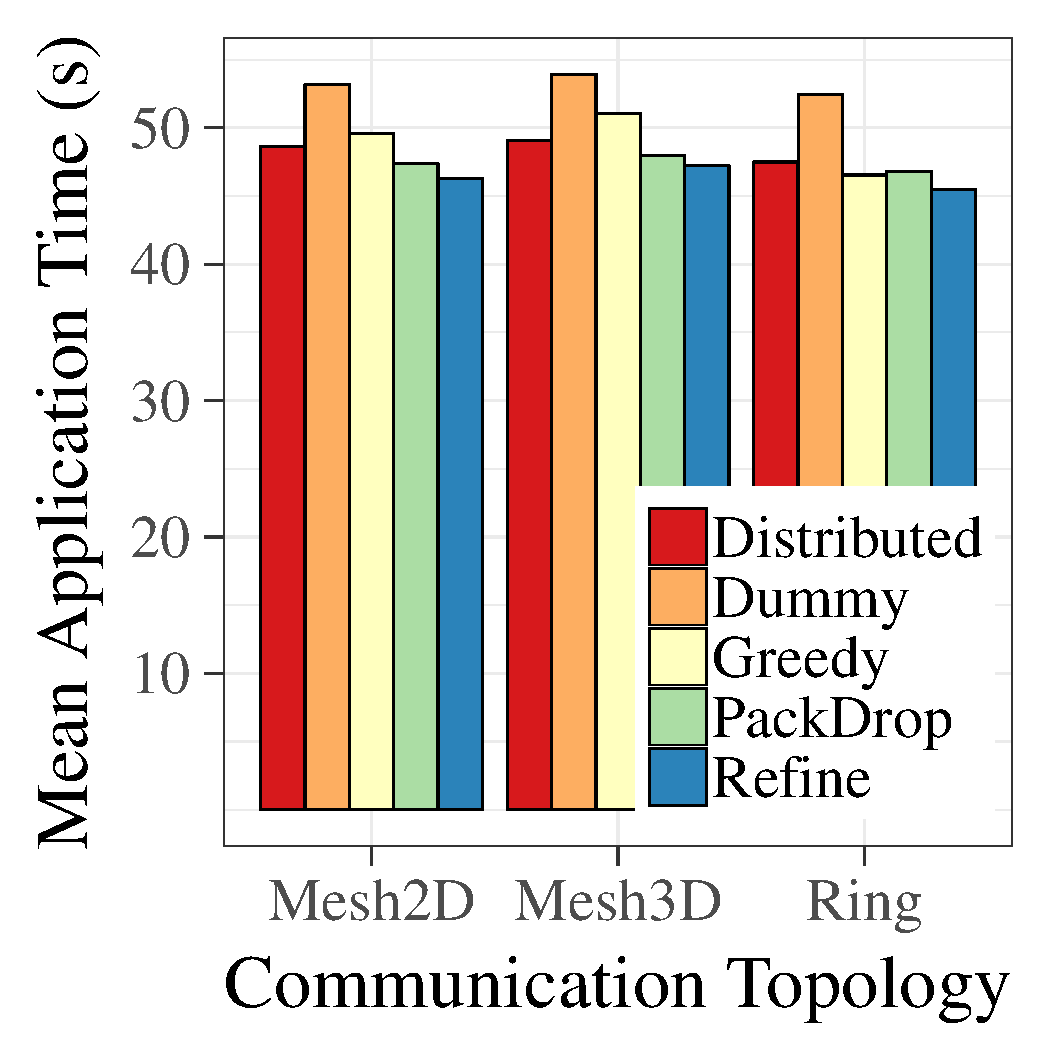
\includegraphics[width=0.4\textwidth]{images/apptime_lbtest_g5k.pdf}
    \caption{LB Test cluster execution results.}
    \label{fig:eval:g5k:lbtest:apptime}
\end{figure}


Each configuration of the benchmark was executed $15$ times, with results depicted on Figure~\ref{fig:eval:g5k:lbtest:apptime} and Table~\ref{tab:lbtest:apptime}.
Results for \textit{Greedy} show how different communication topologies affect the scheduling performance.
Since \textit{Greedy} migrates many \textit{tasks}, the more they communicate, the more migrations impact the application time.

The increased in communication cost can be verified among all scheduling strategies, but in none as much as in \textit{Greedy}.
Our novel approach, \textit{PackDrop} has outperformed the other descentralized strategy, \textit{Distributed}, in the \textit{LB Test} case in this scale.
However, since the platform is not large enough to present all of the potential gains of decentralized strategies, \textit{Refine}, with a reduced migration count approach, still outperforms any other scheduler in this benchmark.
Nevertheless, this indicates a good scalability pontetial, specially in a cluster with high communication overhead, due to its Gigabit Ethernet connection.

\subsubsection*{Evaluation with Molecular Dynamics}

\textit{LeanMD} experiments generated a $9\times9\times9$ space, with a total of $27702$ \textit{tasks}.
Each execution ran $500$ iterations, with a first rescheduling step at the $10$th iteration. 
Rescheduling periods (RP) of every $30$ (short) and every $60$ (long) iterations were used, providing different impacts of rescheduling on the application.
\textit{Greedy} and \textit{Dummy} were excluded from this evaluation due to their high cost in an application such as \textit{LeanMD}. 

\begin{figure}
	\centering
    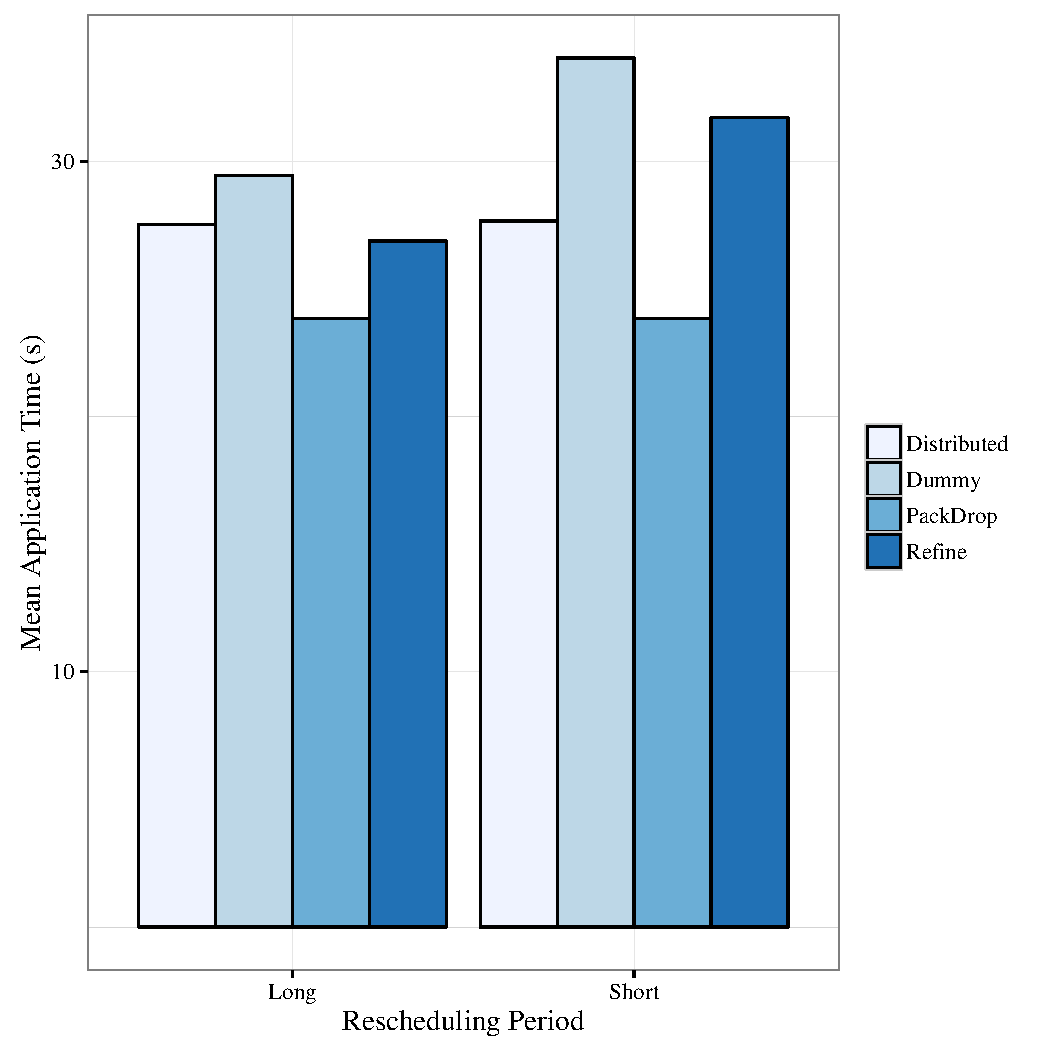
\includegraphics[width=0.4\textwidth]{images/apptime_leanmd_g5k.pdf}
    \caption{LeanMD cluster execution results.}
    \label{fig:eval:g5k:leanmd:time}
\end{figure}

\begin{table}
	\centering
	\begin{tabular}{l|c c}
	Scheduler & Short RP & Long RP \\ \hline
	Distributed & $69.35606$s & $68.36055$s \\ 
	PackDrop & $55.98428$s & $55.51554$s \\ 
	Refine & $59.35696$s & $55.89895$s \\ 
	\end{tabular}
	\caption{LeanMD mean application time on the cluster execution.}	
	\label{tab:eval:g5k:leanmd:time} 
\end{table}

Each configuration of LeanMD was executed $10$ times, making a total of $5000$ steps per configuration and are depicted in Figure~\ref{fig:eval:g5k:leanmd:time} and Table~\ref{tab:eval:g5k:leanmd:time}.
Observed application times presented a standard deviation from the mean lower than $2\%$ for all results presented.



\subsection{Evaluation on Supercomputer}

All experiments executed on supercomputer were compiled with \texttt{Charm++} using the \texttt{--with-production} option, combined with the specifications detailed on Table~\ref{tab:ptinfo}.
Different numbers of homogeneous $2\times 12$ PEs compute nodes ($2$ NUMA-nodes with $12$ cores each) were used to evaluate our strategy's scalability.
We ranged from $16$ ($384$ PEs) to $32$ ($768$ PEs) unique nodes in our evaluation. 

\subsubsection*{Evaluation with Molecular Dynamics}

\textbf{LeanMD} experiments generated a $10\times15\times10$ space, with a total of $171$K \textit{tasks}.
Each execution ran $100$ iterations, with a first rescheduling step at the $9$th iteration. 
Rescheduling was performed every $30$ iterations and each configuration of LeanMD was executed $10$ times, making a total of $1000$ steps per configuration. 

\begin{figure}[!ht]
 \centering
 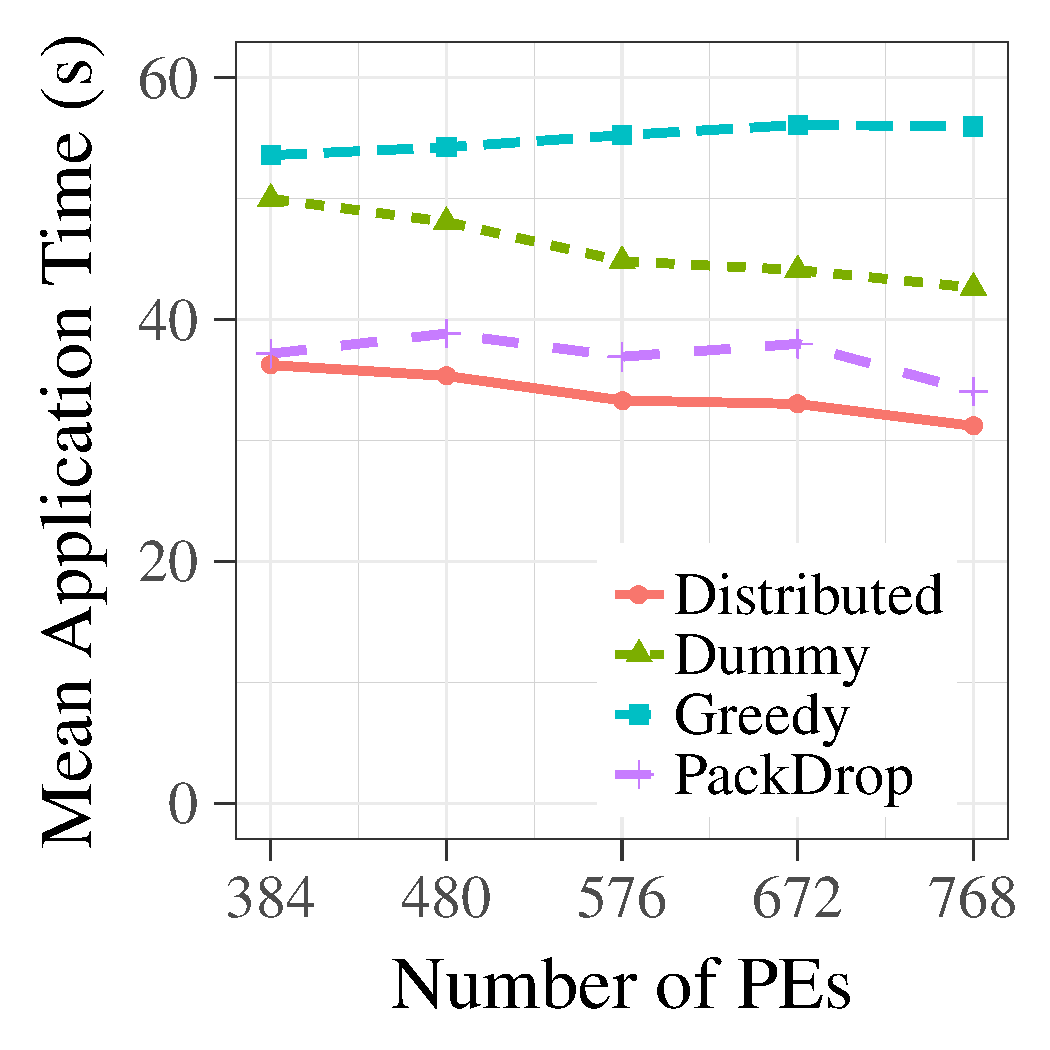
\includegraphics[width=0.9\linewidth]{images/apptime_leanmd_sdumont.pdf}
 \caption{LeanMD supercomputer AppTime execution results.}
 \label{fig:eval:sdumont:leanmd:apptime}
\end{figure}


\begin{figure}
	\centering
	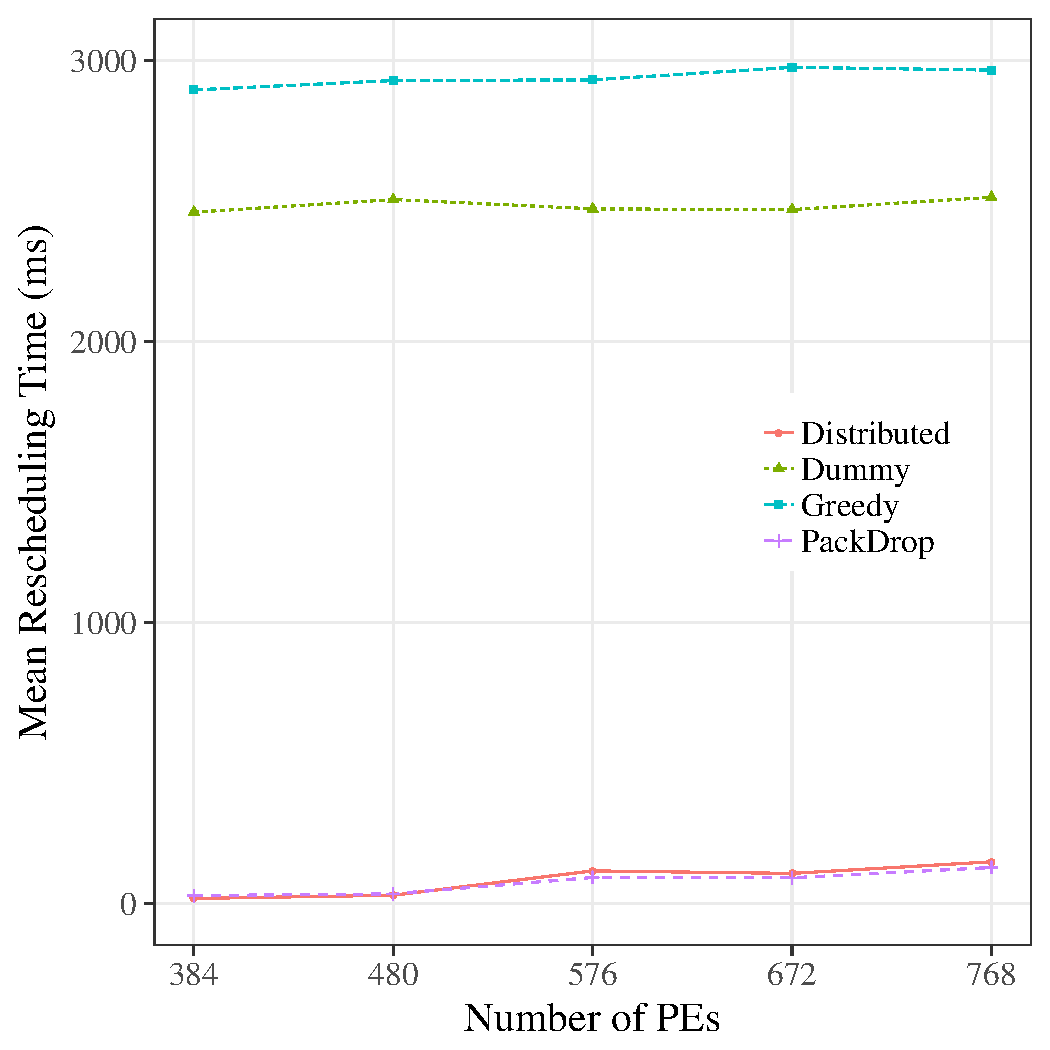
\includegraphics[width=0.9\linewidth]{images/schedtime_leanmd_sdumont.pdf}
	\caption{LeanMD supercomputer SchedTime execution results.}
	\label{fig:eval:sdumont:leanmd:schedtime}
\end{figure}


\subsection{Scalability}